\chapter{Architektur}
\label{cha:architektur}

Die Software-Architektur unserer App musste sich erster Linie den Besonderheiten des Android-Systems anpassen. Dazu wurden neben den Java APIs auch stark die spezifischen Android APIs benutzt. Deren Grundlagen werden wir unten erläutern.

Um die funktionalen Anforderungen zu erfüllen, wurde ein Datenmodell zur Speicherung während der Laufzeit sowie zur persistenten Speicherung benötigt. Die wichtigsten Datenobjekte bei dem Quartett-Spiel sind \emph{Deck} sowie \emph{Card}, wobei ein Deck aus mehreren Karten und eine Karte aus mehreren Bildern sowie Attributwerden besteht. Auf unsere Realisierung des Datenmodells wird unten näher eingegangen.

Eine zentrale funktionale Anforderung ist die Anbindung an einen REST-Server, von dem neue Kartendecks geladen werden können. Die Architektur benötigt also ein Modul, das HTTP-Anfragen senden, textbasierte Daten empfangen und diese in das interne Datenformat umwandeln kann. Unsere Umsetzung davon werden wir unten erklären.

\section{Besonderheiten in Android}
\label{sec:besonderheiten_android}

Eine Android-App setzt sich aus einer oder mehreren \emph{Activities} zusammen. Außerdem ist der App eine \emph{AndroidManifest.xml} Datei zugeordnet, die die enthaltenen Activities deklariert und in eine hierarchische Beziehung zueinander stellt. Activities werden als Java-Klassen implementiert, die von der Klasse \emph{Activity} aus den Android APIs ableiten. Den Einstiegspunkt in die App bildet die \emph{MainActivity}.

\subsection{Activity Lifecycle}

Das Speichermanagement wird vom Android-System im Hintergrund geleistet. Aus Speicherplatz- und Energieeffizienzgründen auf mobilen Geräten haben Activities einen sogenannten Lifecycle. Zu entsprechenden Zeitpunkten werden vom System die Methoden \emph{onCreate()}, \emph{onPause()} usw. aufgerufen (siehe Abbildung \ref{fig:activitylifecycle}). In diese Methoden wird vom Anwendungsprogrammierer Code eingefügt.

\begin{figure}[ht]
\centering
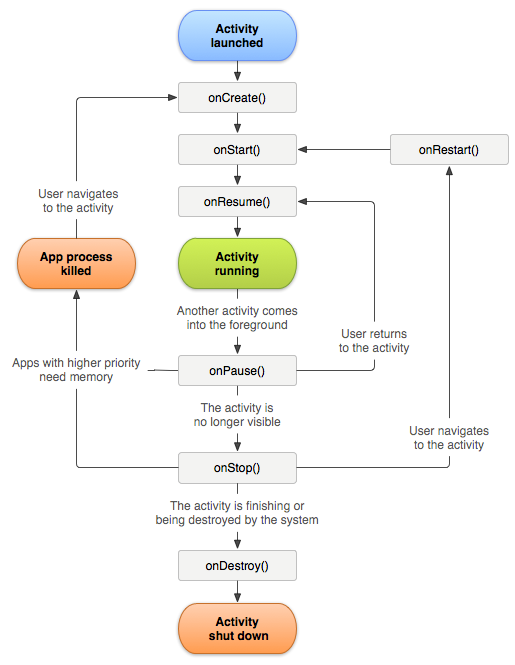
\includegraphics[width=\textwidth]{../img/ActivityLifecycle.png}
\caption{\emph{Activity Lifecycle}}
\label{fig:activitylifecycle}
\end{figure}

\subsection{Layouts und Views}

Um eine GUI anzuzeigen benötigt die Activity ein Layout. Das Layout wird i.d.R. in \emph{onCreate()} mit dem API \emph{setContentView()} gesetzt. Layouts werden in XML Resourcen spezifiziert. Ein Layout enthält hierarchisch angeordnete \emph{Views} (dazu gehören Buttons, TextViews, Checkboxes, ProgressBars, ImageViews usw.). Views erhalten Attribute, die ihre Größe und Position im Layout und ihr Erscheinungsbild festlegen. Außerdem erhalten sie ein ID-Attribut, mit dem in der Activity auf sie zugegriffen werden kann.

Das API \emph{findViewById()} liefert eine Referenz auf die entsprechende View-Instanz. Diese kann nun programmatisch verändert werden. Views implementieren das Observer-Pattern und ermöglichen damit ereignis-orientierte Programmierung. Die Klasse \emph{View} (bzw. davon abgeleitete Klassen) enthalten die APIs \emph{set[Ereignis]Listener()}. Diesen Methoden werden spezielle Listener-Objekte übergeben, die Methoden enthalten, die bei dem entsprechenden Ereignis aufgerufen werden.

\subsection{Kommunikation zwischen Activities}

Zu einem Zeitpunkt ist i.d.R. nur eine Activity aktiv. Beim Wechsel von einer Activity zu einer anderen müssen jedoch Informationen übergeben werden können. Der Wechsel erfolgt zentral durch das API \emph{startActivity()}. Die Methode erhält ein sogenanntes \emph{Intent}-Objekt. Dieses erhält die Informationen in serialisierter Form. Übergibt man ein Java-Objekt, muss dieses also das \emph{Serializable}-Interface implementieren.

\begin{figure}[ht]
\centering
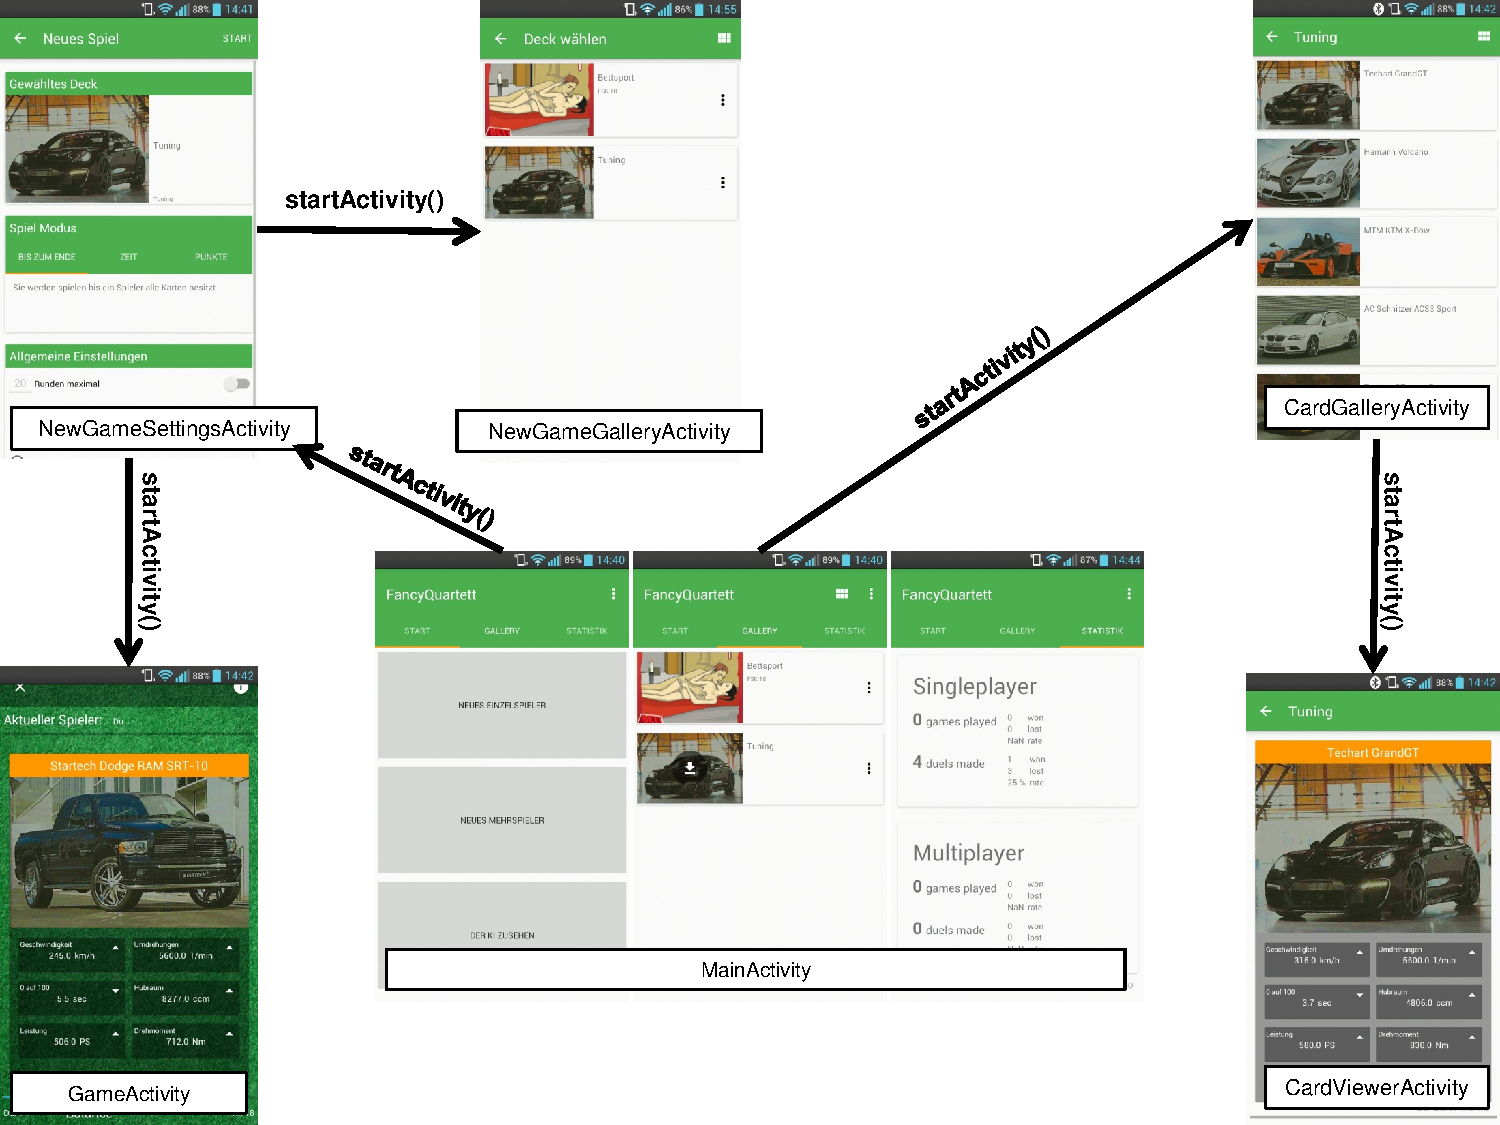
\includegraphics[width=\textwidth]{../img/Activities.pdf}
\caption{\emph{Activities in FancyQuartett}}
\label{fig:activities}
\end{figure}

\section{Datenmodell}
\label{sec:datenmodell}

\section{Netzwerkfunktionen}
\label{sec:netzwerkfunktionen}